\documentclass[aspectratio=149]{beamer}
\usepackage[utf8]{inputenc}

\usepackage[utf8]{inputenc}
\usepackage[T1]{fontenc}

\usepackage[english]{babel}
\usepackage{amsmath}
\usepackage{cleveref}
\usepackage{amssymb}
\usepackage{mathtools}

%%Numbers, expectation
\newcommand{\N}{\mathbb{N}}
\newcommand{\E}{\mathbb{E}}
\renewcommand{\P}{\mathbb{P}}
\newcommand{\Var}{\mathbb{V}}
\newcommand{\R}{\mathbb{R}}
\newcommand{\D}{\mathcal{D}}
\newcommand{\B}{\mathcal{B}}
\newcommand{\Dh}{\D_h}
\renewcommand{\phi}{\varphi}
\newcommand*\diff{\mathop{}\!\mathrm{d}} % integral

%% mathoperator
\DeclareMathOperator*{\argmax}{arg\,max}
\DeclareMathOperator*{\argmin}{arg\,min}
\DeclareMathOperator*{\dom}{dom}
\DeclareMathOperator*{\sign}{sign}
\DeclareMathOperator*{\diag}{diag}

\DeclareMathOperator*{\Cov}{Cov}
\DeclareMathOperator*{\Cor}{Corr}
\DeclareMathOperator*{\Id}{Id}

%proximal operator
\newcommand{\prox}[3][]{\operatorname{prox}^{#1}_{#2}\left(#3 \right)}

\usepackage{xcolor}

%% sort citations by increasing number
\usepackage[sort,nocompress]{cite}

\usepackage{graphicx}% http://ctan.org/pkg/graphicx
\graphicspath{{../figures/}{../../figures}{../../memes}} %Setting the graphicspath
\usepackage{caption,subcaption}

\usepackage{tikz}
\usepackage{pgfplots}
\usetikzlibrary{backgrounds}
\usetikzlibrary{intersections}
\usepgfplotslibrary{fillbetween}

% \usepackage[right]{showlabels}


%%
\theoremstyle{plain}
\newtheorem{prop}{Proposition}[section]
\newtheorem{algo}{Algorithm}[section]
\newtheorem{assumption}{Assumption}
\theoremstyle{remark}
\newtheorem{remark}{Remark}[section]

% cref
\crefname{assumption}{Assumption}{Assumptions}
\crefname{equation}{}{}

\usepackage{autonum}

\usepackage{bm} %% bold math symbols

\usepackage{bbm} %% for \mathbbm{1}


% algorithmic environment
\usepackage{algorithm}
\usepackage[noend]{algpseudocode}

% for some reason this was required on one void linux installation (but not the other)
\usepackage{sansmathaccent}
\pdfmapfile{+sansmathaccent.map}

\author{Axel Böhm}

% shows which section we're in
\usetheme{Darmstadt}

% page number
\setbeamertemplate{footline}[frame number]
\setbeamercolor{page number in head/foot}{fg=gray}


% display things like onslide or visible already before but grayed out
\setbeamercovered{transparent}

% set the itemize item symbol as a diamond
\setbeamertemplate{itemize item}{$\diamond$}
% set the itemize subitem symbol as a triangle
\setbeamertemplate{itemize subitem}{$\blacktriangleright$}

% set the enumerate item symbol as a roman numbers
\setbeamertemplate{enumerate item}{(\roman{enumi})}


\author{Axel Böhm}

% shows which section we're in
\usetheme{Darmstadt}

% page number
\setbeamertemplate{footline}[frame number]
\setbeamercolor{page number in head/foot}{fg=gray}


% display things like onslide or visible already before but grayed out
\setbeamercovered{transparent}

% set the itemize item symbol as a diamond
\setbeamertemplate{itemize item}{$\diamond$}
% set the itemize subitem symbol as a triangle
\setbeamertemplate{itemize subitem}{$\blacktriangleright$}

% set the enumerate item symbol as a roman numbers
\setbeamertemplate{enumerate item}{(\roman{enumi})}


\newcounter{sauvegardeenumi}
\newcommand{\asuivre}{\setcounter{sauvegardeenumi}{\theenumi}}
\newcommand{\suite}{\setcounter{enumi}{\thesauvegardeenumi}}

\title{Acceleration of GD via Momentum}
\date{\today}

\begin{document}
\maketitle
\frame{\tableofcontents}

\section{Optimal methods}

\begin{frame}
  \frametitle{Smooth convex functions: less than $\mathcal{O}(\epsilon^{-1})$ steps?}
  Given $L$ and $D=\Vert x_0 - x^* \Vert$ we know that \textbf{gradient descent}
  \begin{itemize}
    \item converges with $\mathcal{O}(1/k)$
    \item cannot go faster (``lower bound'')
  \end{itemize}

  \begin{block}{}
    \centering
    Maybe GD is not the best possible algorithm? \medskip
  \end{block}


  After all, it is arguably the simplest possible method using the gradient.
\end{frame}


\begin{frame}
  \frametitle{Smooth convex functions: less than $\mathcal{O}(\epsilon^{-1})$ steps?}
  So let's look at the following classes of methods:

  \textbf{First-order} method:
  \begin{itemize}
    \item Access to data only via an \textbf{oracle} returning $f$ and $\nabla f$ at given points.
    \item Clearly, GD is a first order method.
  \end{itemize}

  \begin{block}{}
    \textbf{Q:} What is the \textcolor{blue}{best} first-order method for smooth convex functions.\\
  \end{block}
  \textcolor{gray}{\textit{best}: smallest upper bound on the number of oracle calls \textit{in the worst case}.}

  \begin{itemize}
    \item Nemirovski and Yudin 1979 proved that
          \begin{block}{}
            \center
            every first-order method needs at least $\Omega(1/\sqrt{\epsilon})$ iterations\\
          \textcolor{gray}{to find a point $\bar{x}$ with $f(\bar{x})-f^*\le \epsilon$}.
          \end{block}
  \end{itemize}
  $\Rightarrow$ no method can be faster than $\mathcal{O}(1/k^2)$
\end{frame}


\section{Nesterov momentum}%
\label{sec:}

\begin{frame}
  \frametitle{Acceleration to $\mathcal{O}(1/\sqrt{\epsilon})$ steps}

  \begin{itemize}
    \item Nesterov 1983 proposed a method that needs only $\mathcal{O}(1/\sqrt{\epsilon})$ iterations \textcolor{gray}{(and is therefore the \textit{best one})}.
    \item Known as \textcolor{blue}{\textbf{Nesterov's accelerated gradient}} method.
    \item By now multiple similar algorithms with same complexity exist.
    \item Proofs are generally not really instructive \\
          \textcolor{gray}{(some are computer assisted)}.
  \end{itemize}

\end{frame}


\begin{frame}
  \frametitle{Nesterov's accelerated gradient method}
  \begin{algorithm}[H]
    \caption{Nesterov's accelerated gradient method (NAG)}
    \begin{algorithmic}[1]
      \For{$ k = 0, 1, \dots$}
      \State{$x_{k+1} = y_k - \frac{1}{L} \nabla f(y_k)$}
      \State{$z_{k+1} = z_k - \frac{k+1}{2L} \nabla f(y_k)$}
      \State{$y_{k+1} = \frac{k+1}{k+3} x_{k+1} + \frac{2}{k+3} z_{k+1}$}
      \EndFor{}
    \end{algorithmic}
  \end{algorithm}

  % \begin{align}
  %   x_{k+1} &= y_k - \frac{1}{L} \nabla f(y_k) \\
  %   z_{k+1} &= z_k - \frac{t+1}{2L} \nabla f(y_k) \\
  %   y_{k+1} &= \frac{t+1}{t+3} x_{k+1} + \frac{2}{t+3} z_{k+1}
  % \end{align}

  \begin{itemize}
    \item perform ``\textbf{smooth step}'' from $y_k$ to $x_{k+1}$
    \item perform \textbf{aggressive step} from $z_k$ to $z_{k+1}$
    \item form \textbf{weighted average} of the two\\
          compensate for the aggressive step by giving less weight
  \end{itemize}

\end{frame}

\begin{frame}
  \frametitle{Nesterov's algorithm as a momentum method}
  A different way to write the method is via \textcolor{blue}{momentum}
  \begin{align}
    y_{k} &= x_k + \beta_k (x_k - x_{k-1}) \\
    x_{k+1} &= y_k - \frac{1}{L} \nabla f(y_k).
  \end{align}

  \begin{itemize}
    \item differs from GD only in momentum/inertia term $\beta_k (x_k - x_{k-1})$
    \item has to be chosen carefully $\beta_k = \frac{k-1}{k+2}$
    \item coefficient approaches $\frac{k-1}{k+2} \approx 1 - \frac{3}{k}$
  \end{itemize}
\end{frame}


\begin{frame}
  \frametitle{Nesterov's accelerated gradient method: convergence}
  \textcolor{gray}{Minimum is obtained for $x^*$.}
  \begin{theorem}
    Let $f: R^d \to \R$ be convex and $L$-smooth, then \textbf{NAG} yields
    \begin{equation}
      f(x_k) - f(x^*) \le \frac{2L \Vert x_0-x^* \Vert^2}{\bm{k(k+1)}}
    \end{equation}
  \end{theorem}

  Recall that the gradient descent bound was
  \begin{equation}
      f(x_k) - f(x^*) \le \frac{L \Vert x_0-x^* \Vert^2}{2k}.
  \end{equation}
\end{frame}


\begin{frame}
  \frametitle{$\mathcal{O}(1/k^2)$ vs $\mathcal{O}(1/k)$ in practice}

  \begin{figure}[ht]
    \centering
    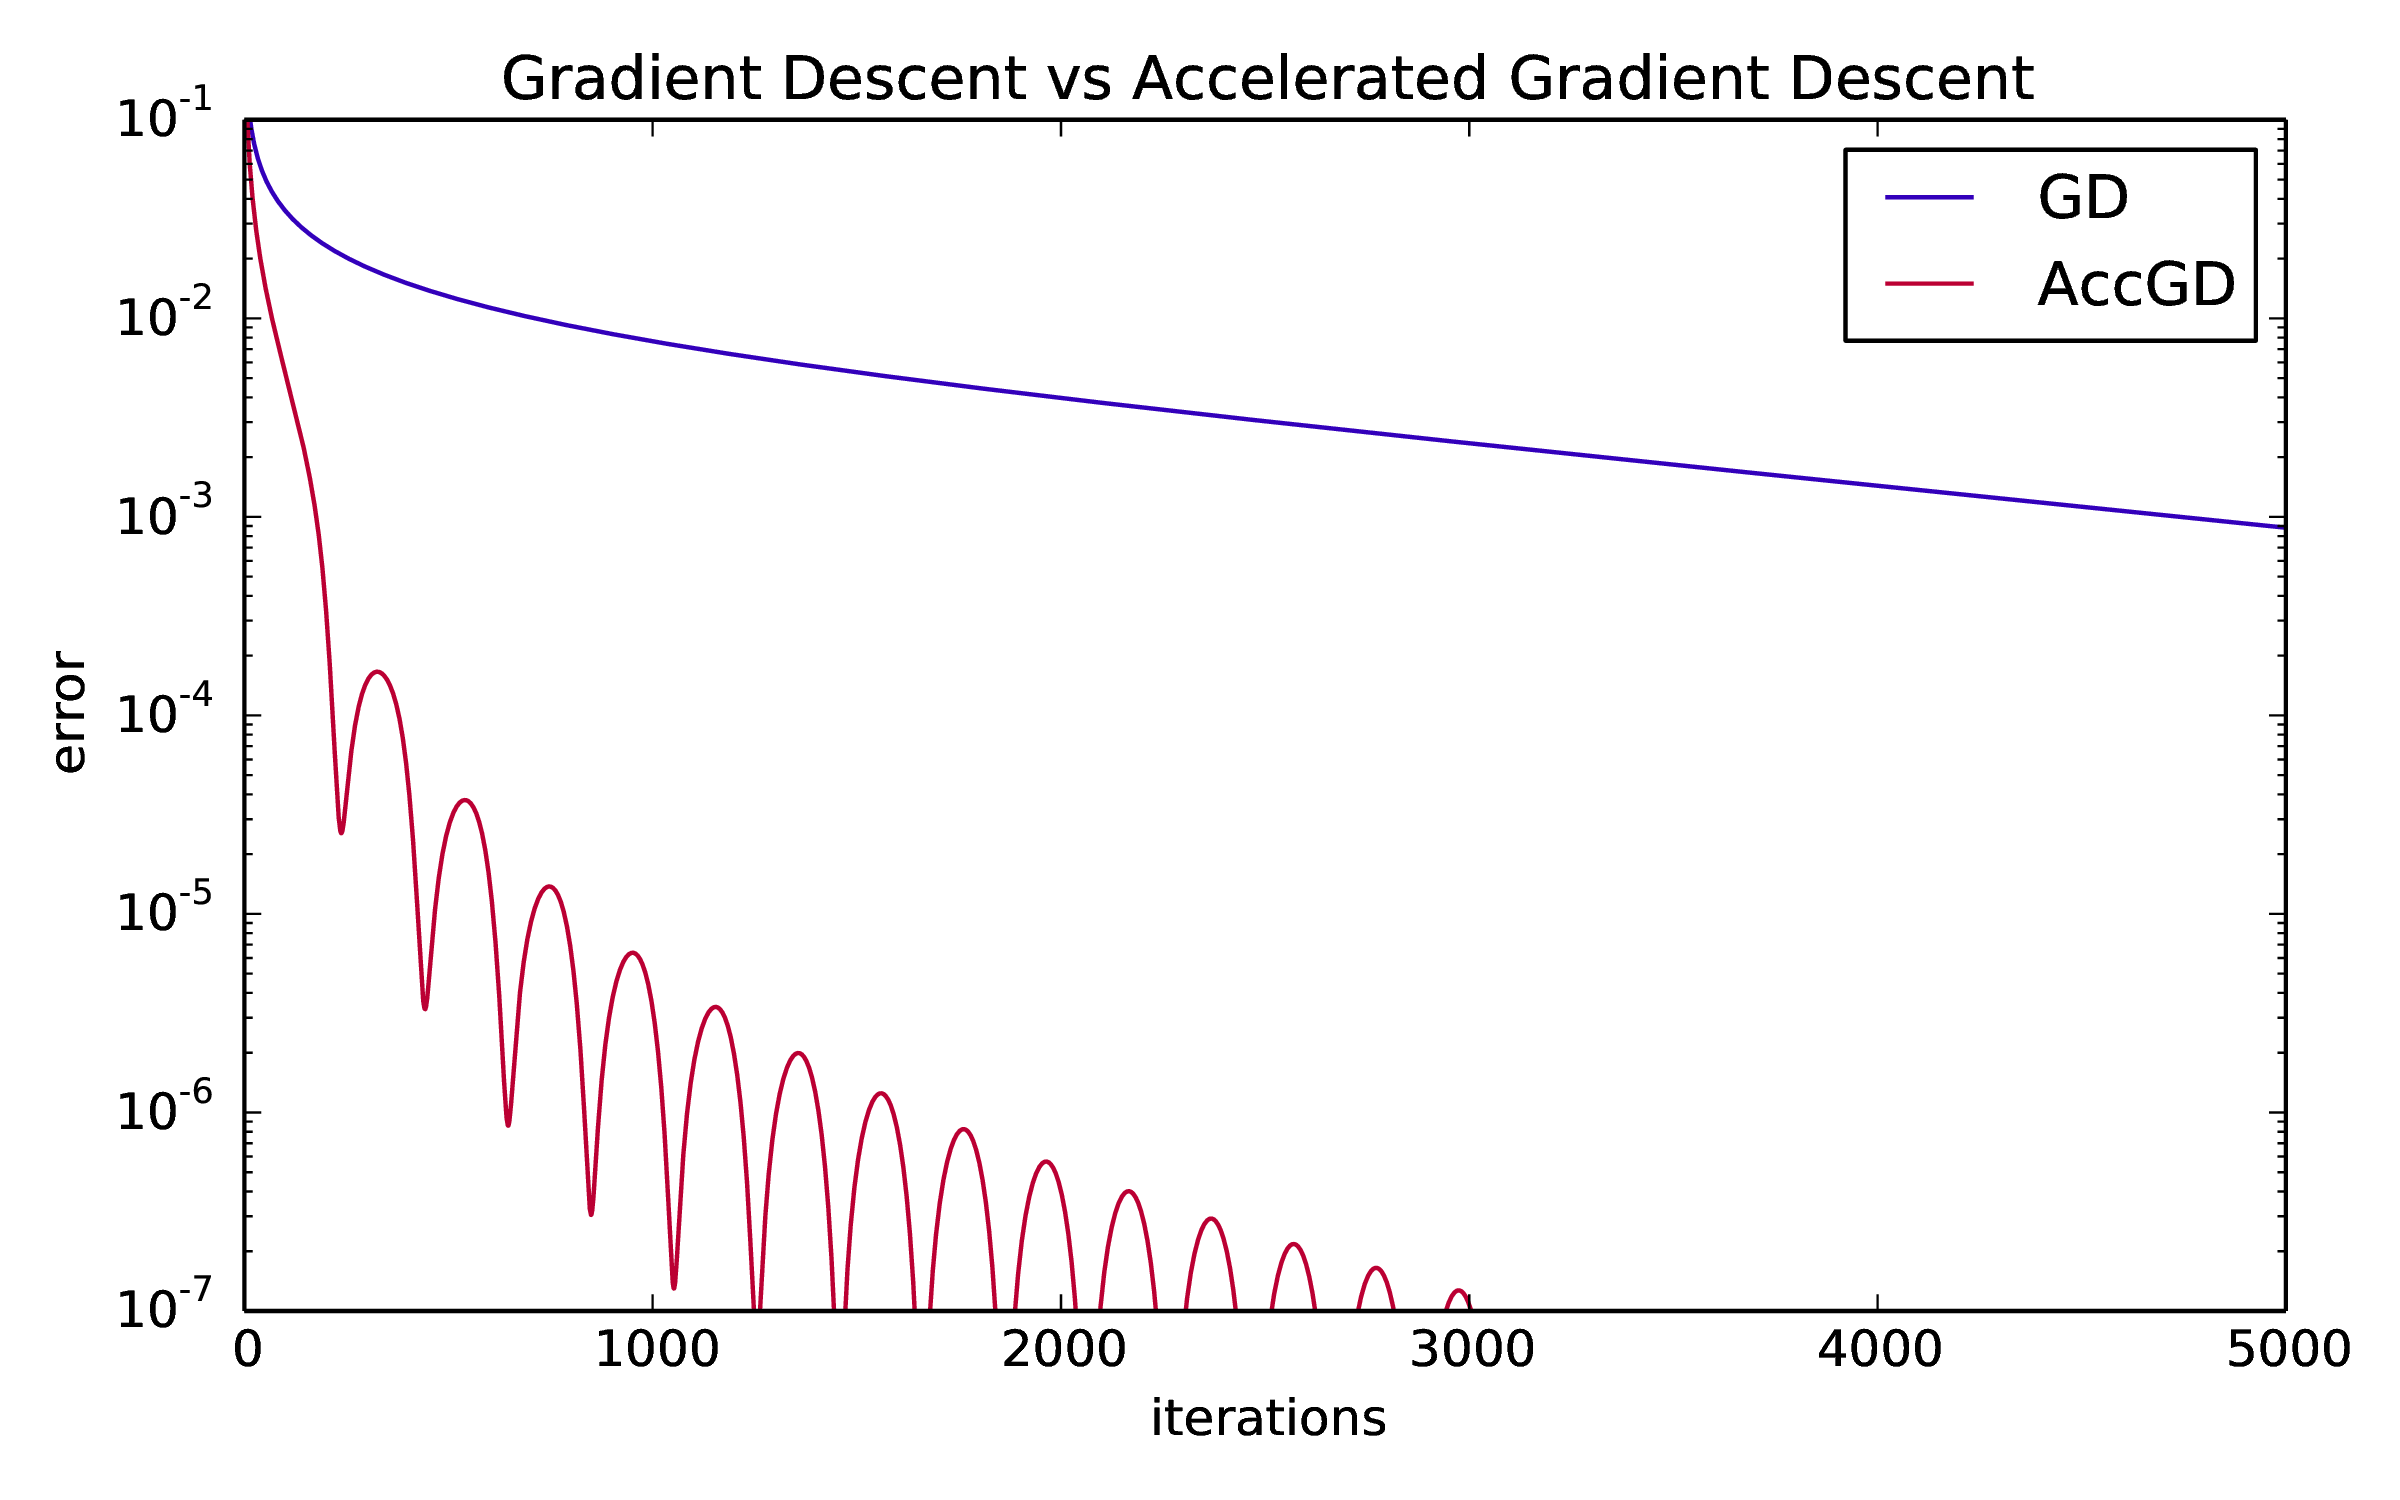
\includegraphics[width=0.9\textwidth,keepaspectratio]{AGD}
  \end{figure}


\end{frame}

\begin{frame}
  \frametitle{Proof idea}
  Potential function $\Phi$ that decreases along trajectory (standard technique).
  Out of the blue: Use
  \begin{equation}
    \Phi(k) := k(k+1) (f(x_k) - f^*) + 2L \Vert z_k - x^* \Vert^2.
  \end{equation}
  Then show that
  \begin{equation}
    \Phi(k+1) \le \Phi(k).
  \end{equation}
  Results in
  \begin{equation}
    \Phi(k+1) \le \Phi(k) \le \cdots \le \Phi(0)
  \end{equation}
  and therefore
  \begin{equation}
    k(k+1) (f(x_k) - f^*)  \le 2L \Vert z_0 - x^* \Vert^2.
  \end{equation}
\end{frame}


\begin{frame}
  \frametitle{Why momentum?}
  \begin{itemize}
    \item GD has problems with \textbf{ravines}, i.e.\ areas where the surface curves much more steeply in one dimension than in another.
    \item Results in zig-zagging.
  \end{itemize}

  \begin{minipage}{0.48\textwidth}
    \begin{figure}[ht]
      \centering
      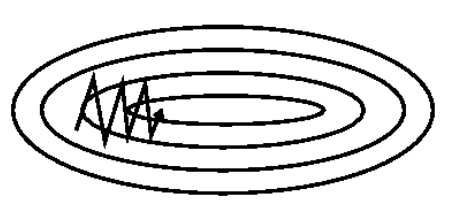
\includegraphics[width=\textwidth,height=\textheight,keepaspectratio]{gd_zig_zag}
      \caption{no momentum}
    \end{figure}
  \end{minipage}
  \begin{minipage}{0.48\textwidth}
    \begin{figure}[ht]
      \centering
      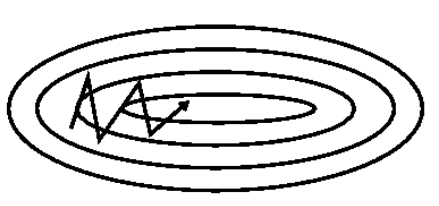
\includegraphics[width=\textwidth,height=\textheight,keepaspectratio]{gd_zig_zag_momentum}
      \caption{with momentum}
    \end{figure}
  \end{minipage}
\end{frame}


\begin{frame}
  \frametitle{Momentum and ravines}
  \begin{figure}[ht]
    \centering
    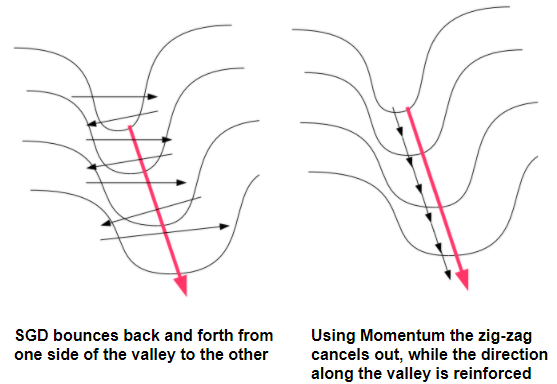
\includegraphics[height=0.9\textheight,keepaspectratio]{ravine-momentum}
    \caption{\label{fig:label} }
  \end{figure}
\end{frame}


\section{Heavy ball}%
\label{sec:}

\begin{frame}
  \frametitle{Momentum in terms of velocity}
  Consider a ball rolling down a slope. Its \textbf{velocity} is
  \begin{align}
    v_k &= \beta v_{k-1} + \alpha \nabla f(x_k) \\
    x_{k+1} &= x_k - v_k
  \end{align}
  \begin{itemize}
    \item a fraction $\beta$ of the \textbf{previous velocity} (friction)
    \item plus, steepness of the \textbf{slope}
  \end{itemize}
  In terms of iterates:
  \begin{align}
    x_{k+1} &= x_k - v_k \\
            &= x_k - \alpha \nabla f(x_k) - \beta v_{k-1} \\
            &= x_k - \alpha \nabla f(x_k) + \beta (x_k - x_{k-1})
  \end{align}
\end{frame}

\begin{frame}
  \frametitle{Heavy ball:  Polyak 1964}
  We derived
  \begin{equation}
    x_{k+1} = x_k - \alpha \nabla f(x_k) + \beta (x_k - x_{k-1}),
  \end{equation}
  while Nesterov's method was
  \begin{align}
    y_{k} &= x_k + \beta_k (x_k - x_{k-1}) \\
    x_{k+1} &= y_k - \frac{1}{L} \nabla f(y_k).
  \end{align}
  However, \textcolor{blue}{\textbf{Polyak's}} momentum provides no speedup over $\mathcal{O}(1/k)$ \\
  \textcolor{gray}{(for smooth convex function)}.
\end{frame}


\begin{frame}
  \frametitle{What's the difference?}
  \begin{itemize}
    \item Both types of momentum seem so similar.
    \item Heavy ball does not care if momentum or gradient first.
    \item Nesterov momentum applies \textcolor{blue}{inertia first}, then gradient:
          \begin{align}
            v_k &= \beta v_{k-1} + \alpha \nabla f(x_k + \beta v_{k-1}) \\
            x_{k+1} &= x_k - v_k.
          \end{align}
          \begin{block}{}
            \center
            Provides stabilization if inertia overshoots.
          \end{block}
  \end{itemize}
\end{frame}

\begin{frame}
  \frametitle{Nesterov vs. Polyak momentum.}
  \vspace{-0.2cm}
  \begin{figure}[ht]
    \centering
    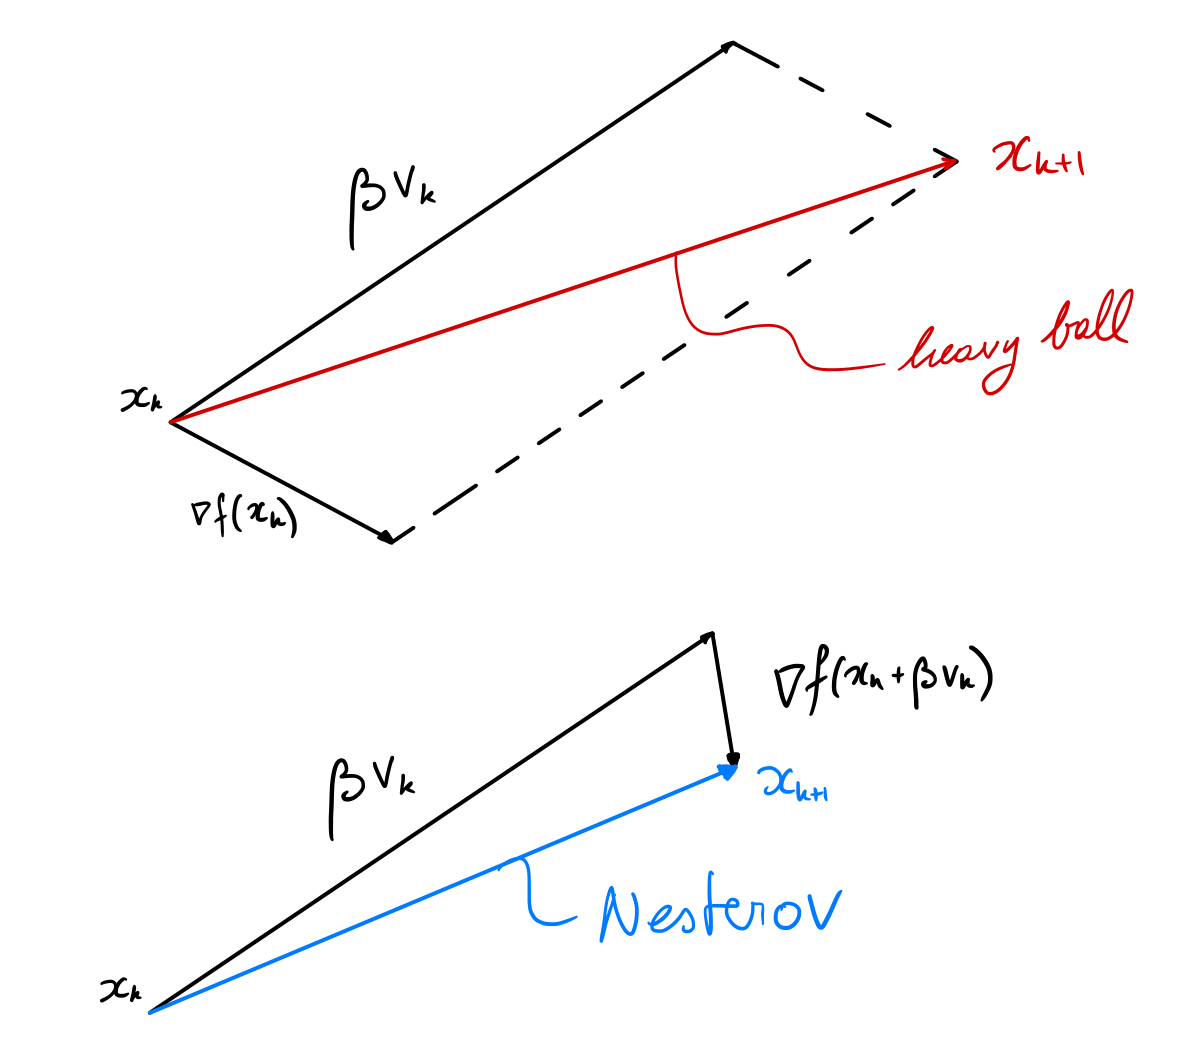
\includegraphics[width=0.6\textwidth,keepaspectratio]{nesterov-vs-polyak2}
  \end{figure}
\end{frame}

\begin{frame}
  \frametitle{Momentum for strongly convex functions}

  For $L$-smooth $\mu$-\textcolor{blue}{strongly convex} we know that GD obtains
  \begin{equation}
    \Vert x_{k+1} - x^* \Vert^2 \le \left(1 - \frac{1}{\kappa}\right) \Vert x_k -x^* \Vert^2
  \end{equation}
  and
  \begin{equation}
    f(x_k)-f^* \le {\left(1-\frac{1}{\kappa}\right)}^k \, \frac{L \Vert x_0 -x^* \Vert^2}{2}.
  \end{equation}
  Performance depends heavily on the \textbf{\textcolor{blue}{condition number}} $\kappa : = L/\mu$.
  $\Rightarrow$ Contraction coefficient is $(1-1/\kappa)$.
  \begin{block}{}
    \center
  Nesterov \textbf{and Polyak} momentum improve this to $(1-1/\sqrt{\kappa})$.
  \end{block}

\end{frame}


\section{when to use}%
\label{sec:}

\begin{frame}
  \frametitle{Momentum for stochastic methods}
  \textbf{\textcolor{blue}{SGD}} analysis can be extended to \textbf{\textcolor{blue}{smooth}} functions with rate
  \begin{equation}
    \mathcal{O}\left(\frac{L}{k} + \frac{\sigma^2}{\sqrt{k}}\right),
  \end{equation}
  where $\sigma^2:= \E [ \Vert \nabla f(x) - g(x) \Vert^2 ]$ is the \textcolor{blue}{variance} of the gradient estimator.

  \medskip
  This can be improved by Nesterov momentum (and additional tricks) to
  \begin{equation}
    \mathcal{O}\left(\frac{L}{k^{\textcolor{red}{2}}} + \frac{\sigma^2}{\sqrt{k}}\right).
  \end{equation}

  Improvement only in the ``\textbf{early phase}'' before noise takes over.

  \begin{block}{}
    \centering
    For worst case rates, only the asymptotic (``late'') phase matters.
  \end{block}
\end{frame}


\begin{frame}
  \frametitle{Momentum and nonsmoothness}
  \begin{itemize}
    \item If $f$ is not differentiable and we have to use subgradients:\\
          no way to improve the $\mathcal{O}(1/\sqrt{k})$ rate.
    \item Works if objective is \textbf{structured}: $f+g$ \textcolor{gray}{(smooth+nonsmooth)}
          \begin{equation}
            \text{FISTA:}\quad \begin{cases}
              y_{k} &= x_k + \beta_k (x_k - x_{k-1}) \\
              x_{k+1} &= \prox{\alpha g}{y_k - \alpha \nabla f(y_k)}.
            \end{cases}
          \end{equation}
          % \begin{align}
          %   y_{k} &= x_k + \beta_k (x_k - x_{k-1}) \\
          %   x_{k+1} &= \prox{\alpha g}{y_k - \alpha \nabla f(y_k)}.
          % \end{align}
          Accelerates from $\mathcal{O}(1/k)$ of proximal-gradient method to $\mathcal{O}(1/k^2)$.
    \item In particular, also works in the \textbf{constrained setting}.
  \end{itemize}

\end{frame}


\begin{frame}
  \frametitle{Momentum in the nonconvex world}
  \begin{itemize}
    \item In theory: difficult to show benefit of momentum for nonconvex problems.
    \begin{itemize}
      \item some statements under additional smoothness assumptions
    \end{itemize}
    \item \textbf{Strong empirical evidence} of usefulness.
        \begin{itemize}
          \item especially in deep learning.
        \end{itemize}
    \item Theory is mostly limited to escaping of saddle points.
  \end{itemize}
\end{frame}


\begin{frame}
  \frametitle{}

  \begin{minipage}{0.3\textwidth}
    \textbf{Momentum in DL:}
  \end{minipage}
  \begin{minipage}{0.6\textwidth}
    \begin{figure}[ht]
      \centering
      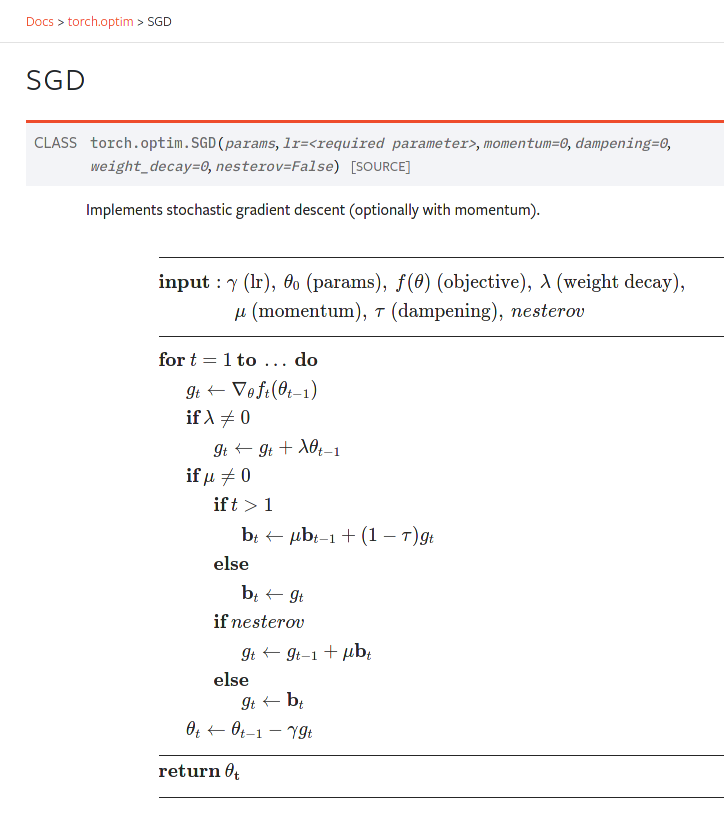
\includegraphics[height=\textheight,keepaspectratio]{sgd-momentum-torch}
    \end{figure}
  \end{minipage}

\end{frame}



\end{document}
